\documentclass[notitlepage]{article}
\usepackage{amsmath,graphicx}
\usepackage[citestyle=numeric,backend=bibtex]{biblatex}
\usepackage[font=small,labelfont=bf]{caption}
\usepackage{verbatim}
\usepackage{pgfplotstable}

\bibliography{library}

\title{Increased concentration of proteins with growth rate can result from passive resource redistribution}
\begin{comment}
\author{Leeat Keren, Uri Barenholz, Ron Milo}
\end{comment}

\begin{document}
\maketitle
\abstract{
  In many microorganisms, the proteome composition changes dramatically as a function of the growth environment.
Furthermore, many of these changes seem to be coordinated with the growth rate rather than the specific environment.
However, although cellular growth rates, gene expression levels and gene regulation have been at the center of biological research for decades, the quantitative interdependence between growth rate and proteome composition is not yet fully understood.

We analyzed the relationship between growth rate and proteome composition for the model microorganism \emph{E.coli} as reflected in two recently published proteomics data sets spanning various growth conditions.
We found that the cellular concentration of a large fraction of the proteins proportionally increases with the growth rate.
This fraction includes proteins that are involved in different cellular processes.
Notably, ribosomal proteins are only a small fraction of this group of proteins.
We present a simple model that demonstrates how such a widely coordinated, proportional, increase in the concentration of many proteins can be the result of passive redistribution of resources, due to active regulation of only a few other proteins.
Our model provides a potential explanation for why and how there is a global coordinated response of a large fraction of the proteome to the growth rate under different environmental conditions.
Its simplicity can also be useful by serving as a baseline null hypothesis in the search for active regulation.

We suggest that, although the concentrations of many proteins change with the growth rate, such changes could be part of a global effect, not requiring specific cellular control mechanisms.
}

\section{Introduction}
A fundamental system-level challenge for cell physiology is the achievement of proper function in the face of various environmental conditions.
It has been established for many years that in different environments cells differ in many properties, including their shape, size, growth rate, and macro-molecular composition \cite{Schaechter1958, Maaloe1969, Churchward1982, Pedersen1978a, ingraham1983growth,Bremer1987}, with strong interdependence between these parameters.

Early on it was found that the expression of some genes is coordinated with growth rate, rather than with the specific environment.
Classical experiments in bacteria, by researchers from what became known as the Copenhagen school, have shown that ribosome concentration (inferred from the RNA to protein ratio in cells) increases in proportion to growth rate\cite{Schaechter1958}.
The search for mechanisms in \emph{E.coli} that underlie this observation yielded several candidates.
Specifically, coordination between ribosome production and growth rate was attributed both to the pools of purine nucleotides \cite{Gourse1996,Gaal1997}, and the tRNA pools through the stringent response \cite{Chatterji2001,Brauer2008a}.
For a more thorough review see \cite{Nomura1984}.
The logic behind this observed increase is that, given that translation rates and active ribosomes fraction remain relatively constant across conditions, a larger fraction of ribosomes out of the proteome is needed in order to achieve faster growth \cite{neidhardt1999a,dennis2004,Zaslaver2009}.

In the last two decades, with the development of the ability to measure genome-wide expression levels, it was found that coordination of gene expression (measured through mRNA levels and promoter-reporter libraries) and growth rate is not limited to ribosomes and ribosomal genes.
In \emph{E.coli}, the expression of catabolic and anabolic genes is coordinated with growth rate, and suggested to be mediated by cAMP \cite{Saldanha2004}.
In \emph{S.cerevisiae}, it was shown that a surprisingly large fraction of the genome changes its expression levels in response to environmental conditions in a manner strongly correlated with growth rate \cite{Keren2013a,Gasch2000,Castrillo2007,Zaslaver2009, Gerosa2013}.
Studies examining the interplay between global and specific modes of regulation, suggested that global factors play a major role in determining the expression levels of genes \cite{Gasch2000, Klumpp2009a,Scott2010, Berthoumieux2013}.
In \emph{E.coli}, this was mechanistically attributed to changes in the pool of RNA polymerase core and sigma factors \cite{Klumpp2008}.
In \emph{S.cerevisiae}, it was suggested that differences in histone modifications around the replication origins \cite{regenberg2006} or translation rates \cite{Gasch2000} across conditions may underlie the same phenomenon.
Important advancements in \emph{E.coli} were achieved by analyzing measurements of fluorescent reporters through a simplified model of gene expression built upon the empirical scaling with growth rate of different cell parameters (such as gene dosage, transcription rate and cell size)\cite{Klumpp2009a}.
These studies suggest that the expression of all genes changes with growth rate, with different architectures of regulatory networks yielding differences in the direction and magnitude of these changes. 

Despite these advancements, many gaps remain in our understanding of the connection between gene expression and growth rate.
Primarily, it is unclear what is the degree of interconnection between gene expression and growth rate.
Is it unique to specific groups of genes or is it a more global phenomenon shared across most genes in the genome?
Genome-wide proteomic data sets, such as those generated by mass-spectrometry, which probe the proteome composition at different growth rates, offer potential insights into these questions.

In this work we analyzed two recently published proteomic data sets of \emph{E.coli} under different growth conditions \cite{Valgepea2013} [ref unpublished Heinemann].
We find a statistically significant positive correlation between growth rate and the protein concentration of many genes, from diverse functional groups.
We present a parsimonious model, which does not require fine-tuning according to organism and condition-specific parameters, that quantitatively predicts the relationship between gene regulation, protein abundance and growth rate.
Our model provides a baseline for the behavior of endogenous genes in conditions in which they are not differentially regulated, on top of which different regulatory aspects can be added.
It suggests that positive correlation of protein concentration with growth rate is a system-emerging property that is the result of passive redistribution of resources, without need for specific regulation mechanisms.

\section{Results}
\subsection{Analysis of proteomic data sets}
To examine the interdependence of protein concentration and growth rate across expressed genes we analyzed two published proteomics data sets of \emph{E.coli}, \cite{Valgepea2013} and [ref Heinemann].
These data sets use mass spectrometry to evaluate the proteomic composition of \emph{E.coli} under $5$ different growth rates using a chemostat, in \cite{Valgepea2013}, and $19$ different growth conditions, spanning both different carbon sources and chemostat-controlled growth rates, in [ref Heinemann].
The [ref Heinemann] data set contains more conditions than those analyzed, see section \ref{heinemanncond} for further details.
\subsubsection{A large fraction of the proteome is positively correlated with growth rate}
For each data set, we calculated the Pearson correlation of every protein with the growth rate.
A histogram of the distribution of the correlations is shown in Figure \ref{fig:growthcorr}.
We find that $\approx 1/3$ of the proteins ($724$ out of $1654$ measured in the data set from [ref Heinemann], hereafter referred to as H, and $296$ out of $919$ in the data set from \cite{Valgepea2013}, hereafter referred to as V) are strongly positively correlated with the growth rate, where a strong correlation with growth rate was defined as a correlation of $R\geq 0.8$ for the V data set, and $R\geq 0.4$ for the H data set.
The thresholds for defining strong correlation with growth rate are the ones maximizing the explained variability in the data (See \ref{corrthreshold} for exact definition and calculation used).
For further comparison and analysis of the causes underlying the differences between the two data sets as reflected in Figure \ref{fig:growthcorr} see section \ref{heinemannchemo}
Notably, in both data sets, the proteins that have a high correlation with the growth rate are involved in different cellular functions and span different functional groups (See tables \ref{tab:corrbreakdownh} and \ref{tab:corrbreakdownv})
Previous studies already found that ribosomal proteins are strongly positively correlated with growth rate (refs).
However, we find that the strongly positively correlated with growth rate group of proteins includes more proteins than the 56 ribosomal proteins, the vast majority of which we also find to be strongly correlated with the growth rate.
Specifically, the proteins that we find to be strongly positively correlated with growth rate are not generally expected to be co-regulated.

\begin{figure}[h]
\centering
\includegraphics{GrowthRateCorrelation.pdf}
\caption{
A large fraction of the proteins have a strong positive correlation with the growth rate in the two data sets analyzed (thresholds used for high correlation are marked in dashed lines).
These proteins span many functional groups.
}
\label{fig:growthcorr}
\end{figure}
\subsubsection{Proteins positively correlated with growth rate share a similar response}
\label{propchange}
Following the identification of the group of strongly positively correlated with growth rate proteins, we examined how similar is the behavior with growth rate for these different proteins.
We note that similar correlation with growth rate for different proteins does not imply that such proteins share the same scaling with growth rate, that is,  they may have very different slopes or fold changes with an increasing growth rate.

In order to compare the responses of different proteins across conditions, we therefore, for every protein, divided its concentration under every condition by its average concentration across all of the conditions (see \ref{concacrossconds} for further details).
This normalized concentration across conditions represents a specific protein, concentration independent, response to the different conditions under which the protein was measured.
We note that, under this metric, sharing similar responses among a group of proteins implies that proteins in that group maintain their relative ratios, ratios that are determined by the average concentration of each of these proteins across the different environmental conditions.
We refer to proteins that share a similar normalized response across different conditions as being coordinated or coordinately regulated.

To assess the coordination between the proteins that were found to be strongly positively correlated with growth rate we therefore calculated the slope of a linear regression line for the normalized concentration vs. the growth rate for every one of these proteins.
The results are presented in Figure \ref{fig:globalfit}, alongside the expected distribution, given the experimental noise in measurements (Further details on the calculation are in section \ref{concacrossconds}).
Further more, we calculated the $95\%$ confidence interval for every slope obtained for any protein.
While the expected distribution of slopes, given the experimental noise, deviates from the observed one, the calculation of confidence intervals reveals that the observed distribution can result from a single response (See SI for further discussion).
These results extend the scope of similar results obtained for \emph{S.cerevisiae} in \cite{Keren2013a} and for expression levels in \emph{E.coli} under stress conditions in \cite{Kaneko2014}.
This analysis thus reveals that, not only is a significant fraction of the proteome strongly positively correlated with the growth rate, but that, as is shown in Figure \ref{fig:globalfit}, this response is coordinated.

Furthermore, we examined how the response of the strongly correlated proteins relates to the well-studied response of ribosomes concentration.
To that end, we performed the same analysis of slopes, restricting it to ribosomal proteins alone, as is shown in Figure \ref{fig:globalfit} (green bars).
We find that, on average, strongly correlated proteins scale in the same way as ribosomal proteins do, implying that the observed response of ribosomal proteins to growth rate is coordinated with a much larger fraction of the proteome, encompassing many more cellular components.
\emph{ToDo: literature survey on mechanisms suggested to control ribosomes concentration to check whether they are for RNA to protein coordination, rRNA to mRNA control, or ribosomal protein control, with our findings highlighting questions on the last ones}.
\emph{ToDo: add statistical test for similarity in response for ribosomal proteins vs all other strongly positively correlated with growth rate proteins}

\begin{figure}[h]
\centering
\includegraphics{AllProtsVSRibosomalNormalizedSlopes.pdf}
\caption{
    A histogram of the slopes of regression lines for every high correlation protein, for the two data sets analyzed.
    Ribosomal proteins are colored in green and non ribosomal proteins in blue.
    To eliminate differences in slopes resulting from different proteins having different average concentrations across conditions, the concentrations for every protein were divided by the average concentration of that protein prior to calculating the linear regression slope (see text for further details).
    The expected distribution of slopes given the experimental noise, assuming all proteins are coordinated, is plotted in red.
    Left panel - data from \cite{Valgepea2013}, right panel - data from \cite{Heinemann2014}.
    High correlation proteins share similar normalized slopes, implying they are coordinated, maintaining their relative ratios across conditions (see text/methods for further details).
    Ribosomal proteins scale with growth rate in a manner similar to the rest of the high correlation proteins.
}
\label{fig:globalfit}
\end{figure}

\subsubsection{Changes in the proteome across environmental conditions are dominated by proteins that are positively correlated with growth rate}
Lastly, we assessed the significance of the positive correlation with growth rate of proteins, out of the total change in proteome composition across conditions.
To that end, we summed the concentrations of all of the proteins that are strongly correlated with growth rate across the conditions measured and plotted their total concentration against the growth rate in Figure \ref{fig:globalgrcorr}.
Both data sets show that the concentration of these proteins change significantly across the different conditions ($\approx 2$ fold change in total concentration across $\approx 5$ fold change of the growth rate).
Moreover, most of the variability of the total concentration of these proteins can be explained by the growth rate ($R^2$ of $0.78$ in H and $0.99$ in V). 
For further analysis of the differences between the two data sets see section \ref{heinemannchemo}.
Importantly, the strongly correlated proteins form a large fraction of the proteome mass-wise, exceeding $50\%$ of the proteome at the higher growth rates measured.
Thus, when considering the changes in proteome composition across conditions, we find that, at higher growth rates, more than $50\%$ of the proteome composition is affected by the positive correlation with growth rate of the same group of proteins.
\emph{ToDo: This analysis, unlike the one done in Leeat's work, does not try to identify the scaling between every two conditions and then cluster genes according to conditions where specific regulation occurred, I'm now thinking of ways of modifying this analysis in that direction as it can potentially be much more interesting and strong so generally I believe this paragraph and accompanying figure will be replaced}

\begin{figure}[h]
\centering
\includegraphics{GlobalClusterGRFit.pdf}
\caption{
The sum of the concentrations of the strongly correlated proteins (defined as having a correlation above 0.8 for the V data set and a correlation above 0.4 for the H data set) in each of the data sets, with linear regression lines, is shown.
These proteins form a large fraction ($>50\%$) out of the proteome at higher growth rates.
The change in the concentration of the strongly correlated proteins follows trend lines with slopes of $\approx 0.5$ meaning their total concentration doubles itself as the growth rate changes by about 5-fold.
Assuming constant degradation rates, these trend lines correspond to protein half life times of 1.5 and 2 hours for the Heinemann and Valgepea data sets respectively.
}
\label{fig:globalgrcorr}
\end{figure}

To conclude, we observe that a large fraction of the change in the proteome composition across conditions is the result of scaling with growth rate of many proteins \emph{ToDo:current estimates are ~ 20 percent at best. Select proper metric and consider if reasonable}.
This scaling with growth rate is coordinated, meaning the proteins maintain their relative abundances.
Finally, this fraction of proteins encompasses many proteins from different functional groups and cellular mechanisms.

\subsection{Theoretical model}
What is the simplest way to explain the observed coordinated growth rate dependence, that is, can this behavior be explained without invoking parameter tuning or complex layers of regulation?
In an attempt to parsimoniously explain this wide-spread, coordinated, positive response, we have constructed a minimalistic model that is able to reproduce these observations as the outcome of redistribution of resources of the bio-synthesis machinery.
Before presenting the model mathematically, we give a brief intuitive depiction.

The model assumes that, under favorable growth conditions, the cell actively down-regulates some proteins that are needed in harsher conditions, as is illustrated in Figure \ref{fig:model}.
As a result, the fraction of each of the rest of the proteins out of the proteome increases, showing the same relative ratios, as long as there is no specific regulation.
The growth rate thus increases, as the ratio of bio-synthetic machinery to the rest of the proteome increases, as is depicted in Figure \ref{fig:model}B.
To demonstrate the idea concretely, one could think about the down regulation of the lac operon in the presence of Glucose, that alleviates the need to transcribe and translate lactose metabolism genes and coincides with faster growth.

\begin{figure}[h]
\centering
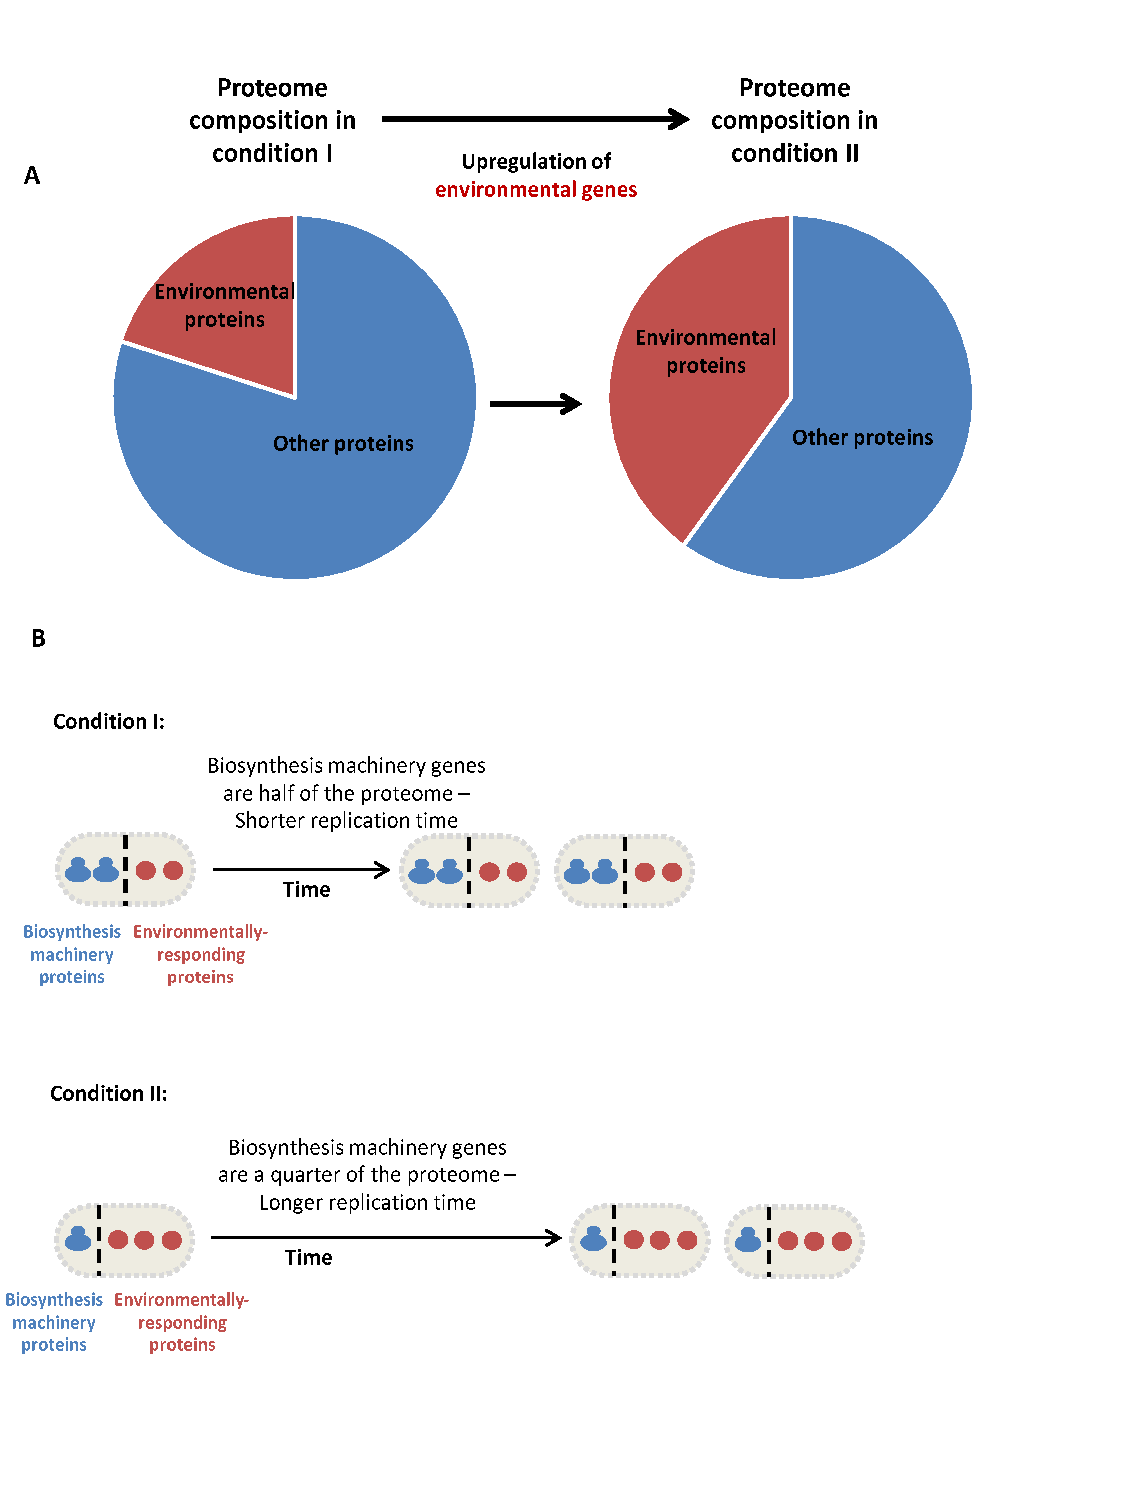
\includegraphics[scale=0.8]{Figures7-trieste.pdf}
\caption{
  A minimalistic model predicts down regulation of environmental genes increases the concentration of other proteins (Panel A).
As a result, the ratio of bio-synthesis machinery genes to the rest of the proteome increases, resulting in faster growth (Panel B).
}
\label{fig:model}
\end{figure}

\subsubsection{The concentration of a protein is determined by both gene specific control, and global expression machinery availability}
For every protein, the model separately considers the resulting concentration as the product of two control mechanisms:
\begin{enumerate}
\item Protein/gene specific controls such as the gene associated promoter sequence, 5'-UTRs, ribosomal binding site sequence, and factors affecting the specific expression of the gene such as transcription factors and riboswitches that react with the relevant gene.
  While some of these controls (such as, for example, the ribosomal binding sites) are static, and therefore condition independent, others are dynamic and may differ under different environmental conditions (such as transcription factors state).
\item The global availability of bio-synthetic resources in the cell, including availability of RNA Polymerase, co-factors, Ribosomes concentration, amino-acids etc.
  All of these factors can potentially differ across different environmental conditions.
\end{enumerate}
For simplicity, the model refers to the fraction of a specific protein out of the proteome, and not to the concentration of that protein in the biomass.
The concentration of a specific protein in the biomass can be calculated given this fraction and the concentration of total protein in the biomass, which is known to be relatively constant \cite{eco-sal} (for further discussion see \ref{protconc}).

According to the model, every gene, under every environmental condition, is given an 'affinity-for-expression' (or 'intrinsic-strength') score that encapsulates its gene-specific control state under the condition considered.
We denote the affinity of gene $i$ under growth condition $c$ by $w_i(c)$ (the notion of affinity for expression is not new, and was first suggested in  \cite{Maaloe1969}).
Our model assumes that the bio-synthetic resources of the cell (Ribosomes, RNA Polymerases, etc.) are distributed among the genes according to their affinities under the condition at hand.
The notion of affinities can thus reduce the number of parameters needed to predict expression levels markedly.
Instead of an expression level for every gene under each condition, there is only a need for the characterization of the affinities a gene may obtain under relevant environmental cues, a parameter set that is expected to be much smaller and easily characterized.
\emph{ToDo: connect to figure showing how coordination serves as a predictor for a gene concentration.}

The resulting protein fraction, under a specific condition, is therefore its specific affinity under the condition, divided by the sum of all the affinities of all of the genes under that same condition.
Thus, if two proteins have the same affinity under some condition, they will occupy identical fractions out of the proteome under that condition.
If protein $A$ has twice the affinity of protein $B$ under a given condition, then the fraction $A$ occupies will be twice as large as the fraction occupied by $B$ under that condition, etc.

This relationship can be simply formulated as follows:
\begin{equation}
  \label{eq:concentration-ratio}
  p_i(c)=\frac{P_i(c)}{P(c)}=\frac{w_i(c)}{\sum_jw_j(c)}
\end{equation}
where $p_i(c)$ denotes the fraction of protein $i$ under condition $c$ out of the proteome, $P_i(c)$ denotes the mass of protein $i$ under condition $c$ per cell, $P(c)$ denotes the total mass of proteins per cell under condition $c$, and the sum, $\sum_jw_j(c)$, is taken over all the genes the cell has.

This equation implies that the observed fraction of a protein is determined by two factors, first, obviously, its own specific affinity that is present in the nominator, but second, and less intuitive and commonly thought of, the affinity of all of the other genes under the growth condition, as reflected by the denominator.

\subsubsection{A change in growth condition triggers changes in expression of specific proteins that indirectly affect all of the proteome}
Different environmental conditions may require the expression of different genes in order to achieve growth.
For example, comparing two growth media, one that includes amino-acids, and one that does not, it can be assumed that when amino-acids are present, no need exists for the cell to express amino-acids synthesizing enzymes, whereas when amino-acids are absent, these enzymes must be expressed.
Therefore, ideally, the cell will be able to sense the presence or absence of amino-acids in the growth media and, for the amino-acids synthesizing genes, down or up regulate their affinities accordingly.
If we now consider some arbitrary gene $i$, whose specific affinity is unaltered between these two conditions, we suggest that, other things being equal, its concentration will still change between the two conditions as the affinities of at least some of the other genes (the amino-acids synthesizing enzymes) change, changing the denominator in equation \ref{eq:concentration-ratio} and thus affecting the distribution of resources between all of the expressed genes.

Generalizing this notion, for every group of conditions, one could divide the proteins into those whose intrinsic affinity remains constant across all of the conditions, and to those whose intrinsic affinity changes (meaning their expression is actively regulated by the cell) between at least some of the conditions, as is shown in Figure \ref{fig:model}A.
An interesting consequence of the formulation in Equation \ref{eq:concentration-ratio} is that proteins whose intrinsic affinities remain constant across different growth conditions, also maintain their relative concentrations across these conditions with respect to each other.
\emph{ToDo: consider adding a panel to Figure 4 to show this, or sub-slices in the blue slice at 4A, or show by writing the equation for the ratio between two proteins whose affinities remain constant, across different conditions}.
Therefore, identifying a large group of proteins that maintain their relative concentrations across conditions (as was identified in section \ref{propchange}) may indicate that these proteins maintain their intrinsic affinities and that any changes in their absolute concentrations are in fact a passive outcome resulting from changes in the intrinsic affinities of other proteins.

\subsubsection{The observed growth rate is an outcome of proteome composition and environmental conditions}
While it is sometimes implied that different cellular components are regulated by the growth rate, here we consider the growth rate as an outcome of the environmental conditions that affect the proteome composition.
Specifically, we arrive at the doubling time as the result of dividing the total amount of proteins per cell by the amount of bio-synthesis machinery in that cell.
The larger the ratio of total proteins to bio-synthesis proteins is, the longer these bio-synthesis proteins will have to operate in order to duplicate the proteome, and thus the longer the doubling time of the cell will be.

To illustrate this assumption concretely, one could think about the total amount of proteins per cell (measured in amino-acids count) divided by the number of ribosomes in the cell.
Assuming each ribosome translates at an approximately condition-independent rate of about 20 amino-acids per second, and as the amount of actively translating ribosomes is also relatively condition-independent \cite{Philips2009} (\emph{ToDo:and its refs}), it follows that the doubling time is linearly dependent on the ratio of proteins to ribosomes in the biomass as illustrated in Figure \ref{fig:model}B.

Theoretically, the fastest doubling time a cell may have is the doubling time achieved when all of the proteome of the cell is the bio-synthetic machinery.
\emph{ToDo - calculate this time based on known rates and molecular sizes and add to SI, check Milo and Philips PNAS paper}
We denote this minimal doubling time by $T_B$.
If the bio-synthetic machinery is only half of the proteome, the doubling time will be $2T_B$ etc.

To integrate the notion of total protein to bio-synthetic protein ratio into our model, we make the following simplifying assumption:
There is a group of bio-synthetic genes (e.g. genes of the transcriptional and translational machineries) the affinities of which remain constant across different growth conditions, a.k.a. these genes are not actively differentially regulated across different conditions.
Furthermore, we assume that the machineries these genes are involved at operate at relatively constant rates and active to non-active ratios across conditions.
Under these assumptions we can define this group of bio-synthesis genes, $G_B$, such that, for every gene that belongs to this group, $k \in G_B$, its affinity, $w_k(c)$ is constant regardless of the condition, $c$.
\begin{equation}
  \label{eq:biosynth-def}
  w_k(c)=w_k
\end{equation}

To keep our notations short, we will define the (condition independent) sum over all of these bio-synthesis genes as the constant: $W_B = \sum_{k\in G_B}w_k$.

As these genes form the bio-synthesis machinery, and according to the assumptions presented above, it follows that the doubling time under a given condition, $\tau(c)$ will be proportional to the ratio of total protein to bio-synthesis protein under that condition, with the proportionality constant being $T_B$:
\begin{equation}
  \label{eq:gr-ratio}
  \tau(c) = T_B\frac{P(c)}{\sum_{k\in G_B}P_k(c)}=T_B\frac{\sum_jw_j(c)}{W_B}
\end{equation}
Therefore, the model implies that for conditions that require the expression of larger amounts of non-bio-synthetic genes (i.e. higher values in the sum over $w_j$ that are not in $W_B$), the resulting doubling time will be longer, i.e., the growth rate will be lower.

\subsubsection{The concentration of a non-differentially regulated protein is expected to increase with the growth rate} 
Recalling that the connection between the growth rate and the doubling time is: $g(c)=\frac{\ln(2)}{\tau(c)}$, we now combine Equation \ref{eq:concentration-ratio} with Equation \ref{eq:gr-ratio} to get that:
\begin{equation}
  \label{eq:default-response}
  p_i(c)=\frac{w_i(c)}{\sum_jw_j(c)}=\frac{w_i(c)}{W_B}\frac{W_B}{\sum_jw_j(c)}=\frac{w_i(c)}{W_B}\frac{T_B}{\ln(2)}g(c)
\end{equation}

Incorporating all the condition-independent constants ($W_B$, $T_B$, $\ln(2)$) into one term, $C$, we get that the predicted fraction of protein $i$ out of the proteome under condition $c$ is:
\begin{equation}
  \label{eq:final-conc}
  p_i(c)=Cw_i(c)g(c)
\end{equation}
which implies that, for every two conditions between which gene $i$ maintains its affinity, ($w_i(c_1)=w_i(c_2)$), the fraction protein $i$ occupies out of the proteome scales like the growth rate change between these two conditions.

To summarize, the simplistic model we have constructed predicts that, under no specific regulation, the fraction a protein occupies out of the proteome should scale with the growth rate.
A group of such proteins should therefore maintain their relative concentrations across conditions.
Finally, when the growth rate approaches zero, the fractions of such proteins, and thus their concentrations, should also approach zero.

However, as the analysis of experimental data in Figure \ref{fig:globalgrcorr} shows, while the concentration of many proteins does indeed scale linearly with growth rate, this scaling does not imply a drop to zero concentration at zero growth.
There are at least two factors that have been neglected in the model, but that can account for this result, and the analysis of their expected effects follows.

\subsubsection{Protein degradation differentiates between measured growth rate and biomass synthesis rate}
Accounting for protein degradation affects the expected concentration of non-differentially regulated proteins at zero growth rate.
Thus, accounting for protein degradation may serve as a partial explanation for the discrepancy between experimental data and predictions made by the model.

Assuming that protein degradation acts on all proteins in the same way, and that it is invariant in the growth condition, the effect of protein degradation can be understood as follows: at any time, some fraction of the entire proteome is degraded.
Therefore, the \emph{observed} growth rate, $g$, is, in fact, the amount of proteins produced \emph{minus} the amount of proteins degraded.
To illustrate, if the measured growth rate is zero, the implication is not that no proteins are produced, but rather that proteins are produced at exactly the same rate as they are degraded.

Integrating this notion into the model means that, where the equations previously referred to the observed growth rate, $g$, as the indicator of protein synthesis rate, they should in fact refer to the observed growth rate plus the degradation rate, as that is the real rate of protein synthesis.
Therefore, if we denote by $\alpha$ the degradation rate (assuming for now equal degradation rates for all genes and under all conditions), Equation \ref{eq:final-conc} should be rewritten as:
\begin{equation}
  \label{eq:final-conc-deg}
  p_i(c)=Cw_i(c)(\alpha+g(c))
\end{equation}
This equation yields better agreement with the experimental results as presented in Figure \ref{fig:globalgrcorr}, depending on the exact value set for degradation.
Degradation can thus explain why the concentration of non-differentially regulated proteins does not drop to zero when the growth rate is zero.
The actual values obtained for the data analyzed are $\alpha=0.34$ for \cite{Valgepea2013} and $\alpha=0.44$ for \cite{Heinemann2014}, corresponding to protein half lives times of $T_{\text{deg}}=2$ hours and $T_{\text{deg}}=1.6$ hours respectively.
As these values correspond to relatively short half lives times, protein degradation is probably only a partial explanation for the differences between the predictions of the model and the observations obtained from the experimental data.

\subsubsection{Slower biological processes rates at slower growth affect the relation between proteome composition and growth rate}
\emph{ToDo - Note that it is an idea Hwa brought up during our conversation}.
The simplistic model assumes that the doubling time is proportional to the ratio of total protein to bio-synthetic protein.
This assumption fails if the rate at which the bio-synthetic machinery operates changes across conditions.
Replacing this assumption by a dependence of bio-synthesis rate with growth rate (such that, the faster the growth, the faster the synthesis rates), will affect the resulting predictions as well.
\emph{ToDo - elaborate and include rigorous definitions as well as experimental evidence, such as increase in $K_{app}$, to the extent that such evidence exists}

\section{Discussion}
We characterized a significant, coordinated response in \emph{E.coli} between many proteins and the growth rate.
This response spans proteins from various functional groups and is not related to the specific medium of growth.
A similar phenomena is observed for \emph{S.cerevisiae} as was reported in \cite{Keren2013a} and may thus be conserved across various organisms and domains of life.
Our analysis suggests that, while changes in the proteome composition may seem complex, they can, to a large extent, be attributed to the linear increase with growth rate of a large number of proteins, at the expense of a few, down-regulated proteins \emph{ToDo: quantify by variation explained}.
The well studied scaling of ribosomes concentration with growth rate can be considered one manifestation of the more general phenomena we describe here.
We find that this response, when considering ribosomal proteins fraction out of the proteome, is not unique and is, in fact, shared with many other proteins spanning different functional groups.

We re-introduce the notion of intrinsic affinity for expression, first presented in \cite{Maaloe1969}, though not widely known.
We show that integrating this notion with the limited bio-synthesis capacity of cells results in a parsimonious mechanism that can explain the response observed in recent experimental data, data that was unavailable at the time this notion was first introduced, nearly 50 years ago.

The framework we present emphasizes the importance of accounting for global factors, that are reflected in the growth rate, when analyzing gene expression and proteomics data.
Specifically, we suggest that the default response of a protein (that is, the change in the observed expression of a protein, given that no specific regulation was applied to it) is to linearly increase with growth rate.
We note that the exact parameters of this dependency may depend on factors such as the degradation rate and the global rate of bio-synthesis mechanisms, as well as the specific affinity of the protein.
We point out that, as non-differentially regulated proteins maintain their relative abundances, one can overcome the lack of knowledge of these factors and use the scaling of most of the proteins in the proteome to infer these expected default dependency parameters \emph{ToDo:have figure demonstrating the connection between the response of a single protein and that of the global cluster or between two proteins that are members of the global cluster. this figure should also illustrate the reduction of parameters obtained by introducing the notion of affinities for expression}

Interestingly, our model demonstrates that no specific control mechanisms need to exist in order to achieve a linear correlation between ribosomal proteins and the growth rate.
However, many such mechanisms have been described before(refs).
We stress that the model does not contradict the existence of such mechanisms.
They may still be needed to achieve faster response under changing environmental conditions or a tighter regulation to avoid unnecessary production and reduce translational noise.
Furthermore, such mechanisms may be crucial for synchronizing the amount of rRNA with ribosomal proteins as the two go through different bio-synthesis pathways.
Nevertheless, the fact that many non-ribosomal proteins share the same response as ribosomal proteins do, poses interesting questions regarding the scope of such control mechanisms, their necessity and the trade-offs involved in their deployment.

\subsection{Relation to other studies}
The findings in this study support and broaden the findings in other recent studies.
Specifically, for \emph{S.cerevisiae} a few recent studies found that the concentration of the majority of the proteins is coordinated across conditions \cite{Keren2013a, Gasch2000, Brauer2008a} and increases with growth rate.\emph{ToDo:verify this for these references and add numbers} 
In principle, the model we suggest here can be applied to any microorganism and may thus also serve as a potential explanation to the phenomena observed in these studies.

Other recently published studies in \emph{E.coli} have suggested different models and in some cases have results  and predictions that do not coincide with those presented in this study.
Notably, in \cite{Klumpp2009a} the opposite behavior for unregulated genes is predicted.
A few differences can explain this seeming discrepancy, among which are different ranges of growth rates observed (the growth rates in this study lie in a range smaller than the growth rates in \cite{Klumpp2009a}), different strains used and very different methods for deducing the expected behavior (ref SI for further discussion?).
\emph{ToDo: consider checking either for genes in the global cluster for which no regulatory elements are expected to exist or replicating similar experiments to those done by Klumpp.} 

Many studies monitored the ribosome concentration in cells and its interdependence with growth rate \cite{Scott2010, Bremer1987, Schaechter1958, 1974, Zaslaver2009, eco-sal}.
While in all of these studies a linear dependence of ribosome concentration with growth rate was observed, in some cases different response strengths were found, compared with the observations in this study.
A discussion for various reasons that may underlie these differences is in \ref{ribosomeconc}.
\emph{ToDo - final paragraph on relation to other works}

\section{Materials and Methods}
Detail data sources, software and algorithms used.
\subsubsection{Normalizing protein concentration across conditions}
\label{concacrossconds}
When comparing the response of different proteins, a normalization is required to compensate for differences in their mean concentrations.
For example, consider two proteins, $A$ and $B$ measured under two conditions, $C_1$ and $C_2$.
Assume that the measured fractions out of the proteome of these two proteins under the two conditions were $0.001$ and $0.002$ for $A$ under $C_1$ and $C_2$ respectively, and $0.01$ and $0.02$ for $B$ under $C_1$ and $C_2$ respectively.
These two proteins therefore respond in the same way across the two conditions, namely, they double their fraction in the proteome in $C_2$ compared with $C_1$.
The normalization procedure scales the data so as to reveal this identity in response.
Thus, once the fraction of each protein out of the proteome is divided by the average fraction of that protein across conditions, we get that the normalized fractions are $\frac{2}{3}$ for both $A$ and $B$ at $C_1$ and $\frac{4}{3}$ for both $A$ and $B$ at $C_2$ showing their identical response.

This normalization procedure has therefore been used prior to calculating the slopes of the regression lines best describing the change in fraction out of the proteome of every protein as a function of the growth rate.
\emph{ToDo: if any other type of clustering is attempted, it should also be noted here that the same normalization was used}
\subsubsection{Filtering out conditions from the Heinemann data set}
\label{heinemanncond}
The [ref Heinemann] data set contains proteomic data measurements under 19 different environmental conditions.
However, some of these conditions are expected to affect the proteome composition in ways not related to the actual growth rate.
Specifically, our model assumes that bio-synthesis rates are condition independent and, at most, change only with growth rate.
That will likely not be the case under specific kinds of conditions such as osmotic pressure, low pH and heat stress.
Additionally, our model assumes exponential growth, implying that measurements taken at stationary phase are expected to differ from simple extrapolation of the model to zero growth rate.
We have therefore omitted such conditions from our analysis and analyzed only those conditions under which our assumptions for bio-synthesis rates being either constant or have a simple relation to the growth rate do hold \emph{ToDo: add these analyses to the SI}.

As, out of the conditions measured in the Heinemann data set, growth in LB media presented a much faster growth rate than the rest of the conditions measured, it dominated the behavior and trends calculated, when included in the analysis.
While including the data on growth in LB does not qualitatively changes the observed results, such analysis is less statistically robust.
We have therefore omitted LB growth data in the main analysis yet present it in the SI.
Including LB growth results in a much smaller set of proteins with a strong positive correlation with growth (as many of the proteins in that group in the slower conditions get down-regulated in LB, significantly reducing their Pearson correlation with growth rate).
On the other hand, the proteins that remain strongly positively correlated with growth rate when LB is included in the analysis show a higher correlation compared with the strongly correlated with growth rate proteins under the slower conditions.
Furthermore, despite the decrease in the number of proteins that are strongly positively correlated with growth when LB is included in the analysis, these proteins form up to $50\%$ of the proteome under LB.

\subsubsection{Calculation of protein concentration}
\label{protconc}
In this study, we use the mass ratio of a specific protein to the mass of the entire proteome, per cell, as our basic measure for the bio-synthetic resources a specific protein consumes out of the bio-synthetic capacity of the cell.
We find this measure to be the best representation of the meaning of a fraction a protein occupies out of the proteome.
However, we note that if initiation rates are limiting, and not elongation rates, then using molecule counts ratios (the number of molecules of a specific protein divided by the total number of protein molecules in a cell) rather than mass ratios may be a better metric.
We compared these two metrics and, while they present some differences in the analysis, they do not qualitatively alter the observed results \emph{ToDo:see SI for comparison}.

There are different, alternative ways to assess the resources consumed by a specific protein out of the resources available in the cell.
On top of the measures detailed above, one could consider either the total mass or molecule count of a specific protein out of the biomass, or out of the dry weight of the cell, both of which take into account the ratio of total protein to biomass or dry weight which was neglected in our analysis.
Moreover, one can consider specific protein mass or molecule count per cell, thus reflecting changes in cell size across conditions.
Our analysis focused on the relations between different proteins and resource distribution inside the proteome, and thus avoided such metrics.
\emph{ToDo - should we justify omitting such analysis?}
\section{Acknowledgments}
(preliminary list) Matthias Heinemann, Stephan Klumpp, Avi Flamholz
\section{Supplementary figures and data}
\subsection{Threshold selection for defining strong correlation with growth rate}
\label{corrthreshold}
The data we use includes the concentrations of proteins under different growth conditions, and the growth rate for every condition.
Given a threshold on the Pearson correlation with growth rate, one can focus on the group of proteins with a correlation with growth rate that is higher than the threshold.
For this group of proteins, a linear regression response can be calculated.
We define the explained variability by the growth rate, given a threshold, as the difference between the total variability of the group of proteins with a correlation higher than the threshold, and the variability remaining, when assuming these proteins scale with the growth rate according to the calculated linear response.
Dividing the explained variability by the total variability of the entire data set quantifies what fraction of the total variability in the data set is explained by considering linear scaling with growth rate for all the proteins with a correlation with growth rate higher than the treshold.
The optimal threshold is then defined as the threshold maximizing this fraction.
Figure \ref{fig:threshold} shows the fraction of the variability explained as a function of the threshold used. 
\begin{figure}[h]
\centering
\includegraphics{ExpVar2.pdf}
\caption{
  Statistics on the explained variability in the data set as a function of the threshold used for defining strong correlation with growth rate.
}
\label{fig:threshold}
\end{figure}

\subsection{Differences between the correlations found in the two data sets}
\label{heinemannchemo}
The lower correlation and higher variability found in the H data set partially results from the variability in the conditions it contains as well as the higher number of conditions measured across a similar rage of growth rates.
Specifically, as this data set includes measurements under different carbon sources, as opposed to the V data set that uses the same carbon source on all measurements, a larger variability in expression patterns is expected.
Restricting the analysis of the H data set only to chemostat conditions supports this suggestion and shows much less variability as is shown in Figure \ref{fig:growthcorrchemo}.
\emph{ToDo consider discussing analysis with LB here or in the SI.}

\subsection{Discussion of reasons for differing ribosome concentration relation to growth rate}
\label{ribosomeconc}
\emph{ToDo: include graph showing ribosome concentration changes across growth conditions both in our data set and data sets from existing literature}
Differences in ribosome concentration  across growth rates as reported in different studies can result from a few factors:
\begin{enumerate}
\item Different growth rates and conditions monitored.
\item Usage of different strains.
\item In many studies the amount of ribosomes is deduced by measuring the RNA to protein ratio, assuming a relatively fixed portion of the RNA is rRNA.
In our study, in contrast, ribosomal proteins are used as a proxy for estimating ribosomes concentration and, moreover, the RNA to Protein ratio is assumed to be constant.
Therefore, and as it is known that ribosomes can operate even in the absence of some ribosomal proteins, such differences in manner of inference can account for some of the differences encountered.
\end{enumerate}

\begin{figure}[h]
\centering
\includegraphics{HeinmannChemostatGr.pdf}
\caption{
  Restricting the analysis of the Heinemann data set to chemostat conditions yields similar results to those of the Valgepea data set.
}
\label{fig:growthcorrchemo}
\end{figure}
\subsection{Unannotated proteins in the Heinemann data set are less correlated with growth than annotated proteins}
Proteins with unknown function (present in Figure \ref{fig:growthcorr}, in the Heinemann data set, right panel) show less correlation with growth rate, as well as proteins with low levels of expression (data not shown).

\subsection{Breakdown by function of proteins strongly correlated with growth rate}
\begin{table}[h]
\centering
%{\hspace*{-4.5cm}
\resizebox{\textwidth}{!}{
\pgfplotstabletypeset[
col sep=semicolon,
columns/Function/.style={string type,column type=l},
columns/totPrctP/.style={column name={$\%$ of proteome}},
columns/corPrctP/.style={column name={Correlated $\%$ of proteome}},
]{funcsHeinemann.csv}
}
\caption{Breakdown by function of the strongly correlated with growth rate proteins in the Heinemann data set.}
\label{tab:corrbreakdownh}
\end{table}

\begin{table}[h]
\centering
%{\hspace*{-4.5cm}
\resizebox{\textwidth}{!}{
\pgfplotstabletypeset[
col sep=semicolon,
columns/Function/.style={string type,column type=l},
columns/totPrctP/.style={column name={$\%$ of proteome}},
columns/corPrctP/.style={column name={Correlated $\%$ of proteome}},
]{funcsValgepea.csv}
}
\caption{Breakdown by function of the strongly correlated with growth rate proteins in the Valgepea data set.}
\label{tab:corrbreakdownv}
\end{table}

\printbibliography
\end{document}